\documentclass[12pt,a4paper]{article}

% ─── Page Layout ───────────────────────────────────────────────────────────────
\usepackage[a4paper, margin=0.8in, headheight=14pt]{geometry}

% ─── Fonts (XeLaTeX) ───────────────────────────────────────────────────────────
\usepackage{fontspec}
\usepackage{unicode-math}
\setmainfont{TeX Gyre Pagella}
\setmonofont[Scale=0.88]{TeX Gyre Cursor}
\setmathfont{Latin Modern Math}

% ─── Packages ──────────────────────────────────────────────────────────────────
\usepackage{xcolor}
\usepackage{colortbl}
\usepackage{titlesec}
\usepackage{enumitem}
\usepackage{tabularx}
\usepackage{booktabs}
\usepackage{array}
\usepackage{amsmath}
\usepackage{tikz}
\usetikzlibrary{shapes.geometric, arrows.meta, positioning, calc, fit, decorations.pathreplacing, patterns, backgrounds}
\usepackage{tcolorbox}
\tcbuselibrary{skins, breakable}
\usepackage{hyperref}
\usepackage{fancyhdr}
\usepackage{graphicx}
\usepackage{microtype}
\hyphenpenalty=10000
\exhyphenpenalty=10000
\sloppy
\usepackage{caption}
\usepackage{setspace}
\usepackage{multirow}
\usepackage{tocloft}

% ─── Q&A helper ────────────────────────────────────────────────────────────────
\newcommand{\Q}[1]{\textbf{#1}\par\noindent\ignorespaces}

% ─── Colour Palette ────────────────────────────────────────────────────────────
\definecolor{myred}{RGB}{196,30,58}
\definecolor{mydark}{RGB}{30,30,50}
\definecolor{mygreen}{RGB}{14,120,80}
\definecolor{myteal}{RGB}{0,130,140}
\definecolor{myamber}{RGB}{180,100,0}
\definecolor{mypurple}{RGB}{100,30,160}
\definecolor{mygray}{RGB}{246,247,249}
\definecolor{mgframe}{RGB}{180,185,200}
\definecolor{watermark}{RGB}{145,150,170}
\definecolor{hdrred}{RGB}{250,232,235}
\definecolor{hdrgreen}{RGB}{220,244,233}
\definecolor{hdrteal}{RGB}{220,242,244}
\definecolor{hdramber}{RGB}{253,242,215}
\definecolor{hdrpurple}{RGB}{238,228,255}
\definecolor{hdrgray}{RGB}{238,240,245}
\definecolor{rowalt}{RGB}{250,251,253}

% ─── Section Formatting ────────────────────────────────────────────────────────
\titleformat{\section}{\large\bfseries\color{myred}}{\thesection.}{0.5em}{}[\vspace{1pt}{\color{myred}\rule{\linewidth}{0.8pt}}]
\titleformat{\subsection}{\normalsize\bfseries\color{myteal}}{\thesubsection}{0.5em}{}
\titlespacing*{\section}{0pt}{18pt}{7pt}
\titlespacing*{\subsection}{0pt}{11pt}{4pt}

% ─── Paragraph ─────────────────────────────────────────────────────────────────
\setlength{\parindent}{0pt}
\setlength{\parskip}{4pt}

% ─── TOC Styling ───────────────────────────────────────────────────────────────
\renewcommand{\cfttoctitlefont}{\large\bfseries\color{myred}}
\renewcommand{\cftaftertoctitle}{\par\noindent{\color{myred}\rule{\linewidth}{0.8pt}}}
\setlength{\cftbeforetoctitleskip}{0pt}
\setlength{\cftaftertoctitleskip}{6pt}
\renewcommand{\cftsecfont}{\normalsize\bfseries\color{mydark}}
\renewcommand{\cftsecpagefont}{\normalsize\bfseries\color{mydark}}
\renewcommand{\cftsecleader}{\cftdotfill{\cftdotsep}}
\setlength{\cftbeforesecskip}{7pt}
\renewcommand{\cftsubsecfont}{\small\color{mydark}}
\renewcommand{\cftsubsecpagefont}{\small\color{mydark}}
\setlength{\cftbeforesubsecskip}{3pt}
\setlength{\cftsubsecindent}{1.4em}

% ─── Table helpers ─────────────────────────────────────────────────────────────
\renewcommand{\arraystretch}{1.45}
\setlength{\tabcolsep}{6pt}
\arrayrulecolor{mydark}
\newcolumntype{B}[1]{>{\small\bfseries\raggedright\arraybackslash}m{#1}}
\newcolumntype{Y}{>{\small\raggedright\arraybackslash}X}
\renewcommand{\tabularxcolumn}[1]{m{#1}}

% ─── Header / Footer ───────────────────────────────────────────────────────────
\pagestyle{fancy}
\fancyhf{}
\fancyhead[L]{\small\color{myred}\textbf{OE-EC804A}\;\color{mydark}--- Artificial Intelligence}
\fancyhead[R]{\small\color{myteal}\textbf{Module 5 Notes}}
\fancyfoot[C]{\small\color{mydark}\thepage}
\fancyfoot[R]{\small\color{watermark}\textit{\copyright\ Biraj Sarkar}}
\renewcommand{\headrulewidth}{0.5pt}
\renewcommand{\footrulewidth}{0.3pt}

% ─── Hyperref ──────────────────────────────────────────────────────────────────
\hypersetup{colorlinks=true, linkcolor=myteal, urlcolor=myteal,
  pdfauthor={Biraj Sarkar}, pdftitle={OE-EC804A --- Module 5 Notes}}

% ─── tcolorbox styles ──────────────────────────────────────────────────────────
\tcbset{
  tikzbox/.style={colback=mygray, colframe=mgframe, boxrule=0.6pt, arc=4pt,
    left=8pt, right=8pt, top=6pt, bottom=6pt,
    colbacktitle=mgframe, coltitle=mydark, fonttitle=\small\bfseries, unbreakable},
  defbox/.style={colback=hdrgreen, colframe=mygreen, boxrule=0.8pt, arc=4pt,
    left=9pt, right=9pt, top=6pt, bottom=6pt,
    colbacktitle=mygreen, coltitle=white, fonttitle=\small\bfseries},
  formulabox/.style={colback=hdrteal, colframe=myteal, boxrule=0.8pt, arc=4pt,
    left=9pt, right=9pt, top=7pt, bottom=7pt,
    colbacktitle=myteal, coltitle=white, fonttitle=\small\bfseries},
  examplebox/.style={colback=hdramber, colframe=myamber, boxrule=0.8pt, arc=4pt,
    left=9pt, right=9pt, top=6pt, bottom=6pt,
    colbacktitle=myamber, coltitle=white, fonttitle=\small\bfseries},
  masonbox/.style={colback=hdrpurple, colframe=mypurple, boxrule=0.8pt, arc=4pt,
    left=9pt, right=9pt, top=6pt, bottom=6pt,
    colbacktitle=mypurple, coltitle=white, fonttitle=\small\bfseries},
  exambox/.style={colback=hdrpurple, colframe=mypurple, boxrule=1pt, arc=5pt,
    left=10pt, right=10pt, top=8pt, bottom=8pt,
    colbacktitle=mypurple, coltitle=white, fonttitle=\bfseries,
    breakable, title after break={\textbf{Frequently Asked / Viva Questions (contd.)}}}
}
\tcbset{breakable}

% ─── TikZ styles ───────────────────────────────────────────────────────────────
\tikzset{
  block/.style={rectangle, draw=myteal, fill=hdrteal, text width=2.4cm, align=center, minimum height=0.9cm, font=\small, rounded corners=3pt},
  arrow/.style={-Stealth, thick, color=mydark},
  line/.style={thick, color=mydark}
}

\begin{document}

% ═══════════════════════════════════════════════════════════════════════════════
% TITLE BLOCK
% ═══════════════════════════════════════════════════════════════════════════════
\begin{center}
  \hfill \textit{Exam-Ready Short Notes} \\
  \vspace{6pt}
  {\LARGE\bfseries\color{myred} OE-EC804A --- Artificial Intelligence}\\[5pt]
  {\normalsize\color{mydark} Semester VIII \quad$\bullet$\quad 3L:0T:0P \quad$\bullet$\quad 3 Credits}\\[3pt]
  {\normalsize\color{myteal}\textbf{Module 5: Knowledge Representation \& Logical Agents}}\\[3pt]
  {\small\color{mydark} CGEC \;$|$\; B.Tech ECE (2023--27) \;$|$\; \textit{Biraj Sarkar}}
\end{center}
\vspace{2pt}
\noindent{\color{myred}\rule{\linewidth}{1.5pt}}
\vspace{2pt}

\hypersetup{linkcolor=mydark}
\tableofcontents
\hypersetup{linkcolor=myteal}
\newpage

% ===============================================================================
\section{Knowledge-Based Agents \& Wumpus World}
% ===============================================================================

\begin{tcolorbox}[defbox, title={Definition of a Knowledge-Based Agent}]
  A \textbf{Knowledge-Based Agent} maintains an internal \textbf{Knowledge Base (KB)} expressed in a formal representation language. It operates by maintaining sentences in its KB, inserting new percepts via \texttt{TELL}, and deriving actions via \texttt{ASK}.
\end{tcolorbox}

\begin{tcolorbox}[formulabox, title={Core Operations of KB Agent}]
  \begin{itemize}[leftmargin=*, noitemsep]
    \item \texttt{TELL(KB, sentence)}: Adds new knowledge or percept to KB.
    \item \texttt{ASK(KB, query)}: Queries KB to infer whether query logically follows from KB.
  \end{itemize}
\end{tcolorbox}

\subsection{The Wumpus World Environment}
The \textbf{Wumpus World} is a benchmark domain for logical reasoning.
\begin{itemize}[leftmargin=*, itemsep=3pt]
  \item $4 \times 4$ grid of rooms containing a Wumpus, Pits, and Gold.
  \item \textbf{Percepts:} $[Stench, Breeze, Glitter, Bump, Scream]$.
  \item \textbf{Rules:} Rooms adjacent to Wumpus have $Stench$. Rooms adjacent to Pits have $Breeze$. Room containing Gold has $Glitter$.
\end{itemize}

\begin{tcolorbox}[tikzbox, title={Wumpus World Grid Environment ($4 \times 4$)}]
\centering
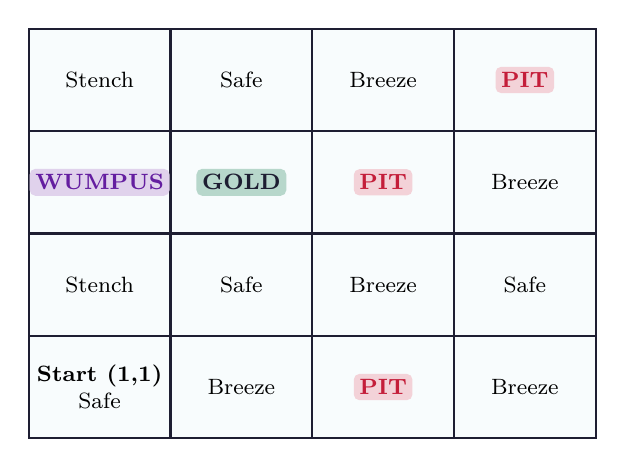
\begin{tikzpicture}[x=1.8cm, y=1.3cm]
  \draw[line, fill=hdrteal!20] (0,0) rectangle (4,4);
  \draw[line, step=1] (0,0) grid (4,4);
  
  % Row 1 (y=0.5)
  \node[align=center, font=\footnotesize] at (0.5,0.5) {\textbf{Start (1,1)}\\Safe};
  \node[align=center, font=\footnotesize] at (1.5,0.5) {Breeze};
  \node[align=center, font=\footnotesize, fill=myred!20, inner sep=2pt, rounded corners=2pt] at (2.5,0.5) {\textbf{\color{myred}PIT}};
  \node[align=center, font=\footnotesize] at (3.5,0.5) {Breeze};
  
  % Row 2 (y=1.5)
  \node[align=center, font=\footnotesize] at (0.5,1.5) {Stench};
  \node[align=center, font=\footnotesize] at (1.5,1.5) {Safe};
  \node[align=center, font=\footnotesize] at (2.5,1.5) {Breeze};
  \node[align=center, font=\footnotesize] at (3.5,1.5) {Safe};
  
  % Row 3 (y=2.5)
  \node[align=center, font=\footnotesize, fill=mypurple!20, inner sep=2pt, rounded corners=2pt] at (0.5,2.5) {\textbf{\color{mypurple}WUMPUS}};
  \node[align=center, font=\footnotesize, fill=mygreen!30, inner sep=2pt, rounded corners=2pt] at (1.5,2.5) {\textbf{\color{mydark}GOLD}};
  \node[align=center, font=\footnotesize, fill=myred!20, inner sep=2pt, rounded corners=2pt] at (2.5,2.5) {\textbf{\color{myred}PIT}};
  \node[align=center, font=\footnotesize] at (3.5,2.5) {Breeze};
  
  % Row 4 (y=3.5)
  \node[align=center, font=\footnotesize] at (0.5,3.5) {Stench};
  \node[align=center, font=\footnotesize] at (1.5,3.5) {Safe};
  \node[align=center, font=\footnotesize] at (2.5,3.5) {Breeze};
  \node[align=center, font=\footnotesize, fill=myred!20, inner sep=2pt, rounded corners=2pt] at (3.5,3.5) {\textbf{\color{myred}PIT}};
\end{tikzpicture}
\end{tcolorbox}

% ===============================================================================
\section{Propositional Logic}
% ===============================================================================

Propositional logic represents facts using proposition symbols ($P, Q, R$).

\begin{tcolorbox}[defbox, title={Logical Entailment}]
  Sentence $\alpha$ \textbf{entails} sentence $\beta$ ($\alpha \models \beta$) if and only if in every model in which $\alpha$ is true, $\beta$ is also true.
\end{tcolorbox}

\subsection{Logical Equivalences}
\par\vspace{6pt}\noindent
{\renewcommand{\arraystretch}{1.4}%
\begin{tabularx}{\linewidth}{|B{3.5cm}|Y|}
\hline
\textbf{Equivalence Law} & \textbf{Formula} \\
\hline
Implication Elimination & $\alpha \implies \beta \equiv \neg \alpha \lor \beta$ \\
\hline
Biconditional Elimination & $\alpha \iff \beta \equiv (\alpha \implies \beta) \land (\beta \implies \alpha)$ \\
\hline
De Morgan's Laws & $\neg(\alpha \land \beta) \equiv \neg \alpha \lor \neg \beta \quad ; \quad \neg(\alpha \lor \beta) \equiv \neg \alpha \land \neg \beta$ \\
\hline
Distributivity & $\alpha \land (\beta \lor \gamma) \equiv (\alpha \land \beta) \lor (\alpha \land \gamma)$ \\
\hline
\end{tabularx}}

% ===============================================================================
\section{Inference \& Resolution in Propositional Logic}
% ===============================================================================

\subsection{Resolution Rule}
Unit Resolution rule states that:
\begin{equation}
  \frac{l_1 \lor l_2 \lor \dots \lor l_k, \quad \neg l_i}{l_1 \lor \dots \lor l_{i-1} \lor l_{i+1} \lor \dots \lor l_k}
\end{equation}

Resolution Refutation proves $KB \models \alpha$ by showing that $KB \land \neg \alpha$ is \textbf{unsatisfiable}.

\subsection{Conjunctive Normal Form (CNF) Conversion Steps}
\begin{enumerate}[leftmargin=*, itemsep=3pt]
  \item Eliminate $\iff$ replacing $\alpha \iff \beta$ with $(\alpha \implies \beta) \land (\beta \implies \alpha)$.
  \item Eliminate $\implies$ replacing $\alpha \implies \beta$ with $\neg \alpha \lor \beta$.
  \item Move $\neg$ inwards using De Morgan's laws ($\neg(\alpha \lor \beta) \equiv \neg \alpha \land \neg \beta$).
  \item Distribute $\lor$ over $\land$ ($\alpha \lor (\beta \land \gamma) \equiv (\alpha \lor \beta) \land (\alpha \lor \gamma)$).
\end{enumerate}

\newpage
\begin{center}
  {\large\bfseries\color{myred} Quick Revision --- Module 5}\\[3pt]
  {\small\color{mydark} Knowledge Representation \& Logical Agents $|$ OE-EC804A}
\end{center}
\noindent{\color{myred}\rule{\linewidth}{1.2pt}}
\vspace{4pt}

\begin{tcolorbox}[formulabox, title={\textbf{Key Concepts and Metrics at a Glance}}]
\renewcommand{\arraystretch}{1.35}
\begin{tabularx}{\linewidth}{B{4.5cm} X}
Logical Entailment & $KB \models \alpha \iff M(KB) \subseteq M(\alpha)$ \quad ($\alpha$ true in all KB models) \\[4pt]
Proof by Contradiction & $KB \models \alpha \iff (KB \land \neg \alpha)$ is unsatisfiable \\[4pt]
Implication Elimination & $\alpha \implies \beta \equiv \neg \alpha \lor \beta$ \\[4pt]
Resolution Rule & $\frac{\alpha \lor \beta, \quad \neg \beta \lor \gamma}{\alpha \lor \gamma}$ \quad (Derives empty clause on contradiction) \\[4pt]
CNF Structure & Conjunction of disjunctions of literals (AND of OR clauses) \\
\end{tabularx}
\end{tcolorbox}

\begin{tcolorbox}[defbox, title={\textbf{One-Line Definitions}}]
  \begin{itemize}[leftmargin=*, noitemsep]
    \item \textbf{Knowledge Base (KB):} A set of sentences expressed in a formal representation language.
    \item \textbf{Model:} A mathematical world assigning truth values (True/False) to every proposition.
    \item \textbf{CNF:} A conjunction of disjunctions of literals (AND of ORs).
    \item \textbf{Sound Inference:} Derives only entailed sentences (no false conclusions).
    \item \textbf{Complete Inference:} Can derive any sentence that is entailed.
  \end{itemize}
\end{tcolorbox}

\begin{tcolorbox}[exambox, title={\textbf{Frequently Asked / Viva Questions}}]
  \begin{enumerate}[topsep=0pt, label=\textbf{Q\arabic*.}, itemsep=5pt]
    \item \Q{Define a Knowledge-Based Agent.}
    An agent that reasons over a formal Knowledge Base (KB) using TELL and ASK operations to select actions.

    \item \Q{What is Entailment ($\models$)?}
    $KB \models \alpha$ means $\alpha$ is true in all models where KB is true.

    \item \Q{What is the difference between Syntax and Semantics?}
    Syntax defines allowable sentence structures. Semantics defines sentence meaning and truth values in models.

    \item \Q{State De Morgan's Laws.}
    $\neg(P \land Q) \equiv \neg P \lor \neg Q$ and $\neg(P \lor Q) \equiv \neg P \land \neg Q$.

    \item \Q{What is Conjunctive Normal Form (CNF)?}
    A logical sentence format structured as an AND of clauses, where each clause is an OR of literals.

    \item \Q{How does Resolution Refutation work?}
    To prove $KB \models \alpha$, add $\neg \alpha$ to KB and apply resolution rules until an empty clause (contradiction) is derived.

    \item \Q{Differentiate Soundness and Completeness.}
    Soundness: Everything derived is true ($KB \vdash \alpha \implies KB \models \alpha$). Completeness: Every true fact can be derived ($KB \models \alpha \implies KB \vdash \alpha$).

    \item \Q{What is Forward Chaining?}
    An inference algorithm for Horn clauses that starts from known facts and applies rules to infer new facts until query is proved.

    \item \Q{What is Backward Chaining?}
    An inference algorithm that starts from query goal and works backward through rules to find supporting facts.

    \item \Q{What is a Horn Clause?}
    A disjunction of literals containing at most one positive literal.
  \end{enumerate}
\end{tcolorbox}

\end{document}
